% Note that if you want something in single space you can go back and
% forth between single space and normal space by the use of \ssp and
% \nsp.  If you want doublespacing you can use \dsp.  \nsp is normally
% 1.5 spacing unless you use the doublespace option (or savepaper
% option)
%
%(FORMAT) Usually you *don't* want to mess with the spacing for your
%(FORMAT) final version.  If you think/know that the thesis template
%(FORMAT) and/or thesis style file is incorrect/incomplete, PLEASE
%(FORMAT) contact the maintainer.  THANK YOU!!!

\chapter{ESSENTIAL CONTRIBUTIONS OF THIS THESIS}
\label{chap:binarysearchtree}
% By labeling the chapter, I can refer to it later using the
% label. (\ref{chap:binarysearchtree}, \pageref{chap:binarysearchtree}) Latex will take care
% of the numbering.

\section{Crux of the thesis} 

The main research topic of this thesis is to optimize the time required to compute the neighnor in an AVL tree. We have studied uptil now the original algorithm as given in the text book \cite{TEXTBOOK1}. One of the goals of this thesis research is to present a traditional working algorithm for academic purpose. Also besides implementing the original algorithm, the main contribution of this thesis research is to modify one of the data structure used in to original algorithm with an intention to optimize it. By doing so we will present an optimized version of the algorithm.

As we have already seen till now we are using an AVL tree to maintain the status structure and event queue. One of the most frequently required operations for these data structures is to compute the adjacent left and right neighbor�s. With the traditional implementation of an AVL tree suppose we search in the tree for the segment immediately to the left of some segment �L1� that lies on the sweep line. At each internal node �V� starting from root node we first need to find the leaf node �L1�. Thus at each internal node �V� we test whether �L1� lies to the left or right of the segment stored at the internal node. Depending on the outcome we descend to the left or right of the segment stored at �V� eventually ending up in the leaf node �L1�. Now since we need to find the left neighbor of �L1� we first need to traverse to the common parent between �L1� and its left neighbor. After that we need to descend downwards to get the left neighbor of �L1�. Similar strategy is to be followed but exactly in the opposite direction for finding the next right neighbor. This would take{\it O}(log n) time and is a very costly operation. This would be worst if the neighbor lies in an entirely different subtree and would require us to traverse back to the root and then descend again downwards in the direction of the neighbor.
\begin{figure}[ht]
  \begin{center}
   	\fbox{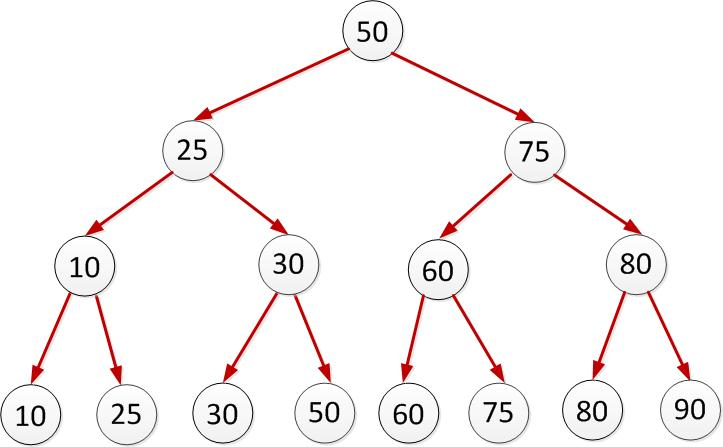
\includegraphics[width=6in, height=2.75in]{Figures/Figure22}}
  \end{center}
  \centering
	\parbox{6in}{\caption{A typical balanced AVL tree.} \label{fig22}} 
\end{figure}

For instance consider Figure.~\ref{fig22}. Suppose we need to find the left neighbor of 50. We would start with the root node 50 and descend towards left as search node �50� is equal to the root node 50. Then we would come at node 25. After which we would move right downward as 50 is greater than 25. Thus we would reach node 30 and finally at 50 which is the leaf node. But we wanted to get the left neighbor of 50, so we would again move upward to 30 which happen to be the common parents between leaf node 50 and its left neighbor. Then we would move down left to get 30, which is the left neighbor, which is the actual node that we were searching. Now suppose we wanted to find the right neighbor of 50 then we would start at root node and traverse 50-25-30-50 as before. But since we wanted the right neighbor, we would have to first traverse to the common parent between leaf node 50 and its right neighbor.  Thus we would again traverse all the way upwards starting at leaf node 50 with the path 50-30-25-50 and then move right to follow the path 75-60-60 to finally get the right neighbor of 50. This would be a very costly operation if the depth of the tree is huge.

It would certainly be better if we could optimize this time as this is the most frequently used operation in the algorithm. This thesis is proposing an elegant solution where this searching can be optimized. As the tree is built this thesis proposes to store the left and right pointers only in the leaf nodes. These pointers would be continuously updated whenever a new node is inserted or deleted in the tree (Figure.~\ref{fig23}).  
\begin{figure}[ht]
  \begin{center}
   	\fbox{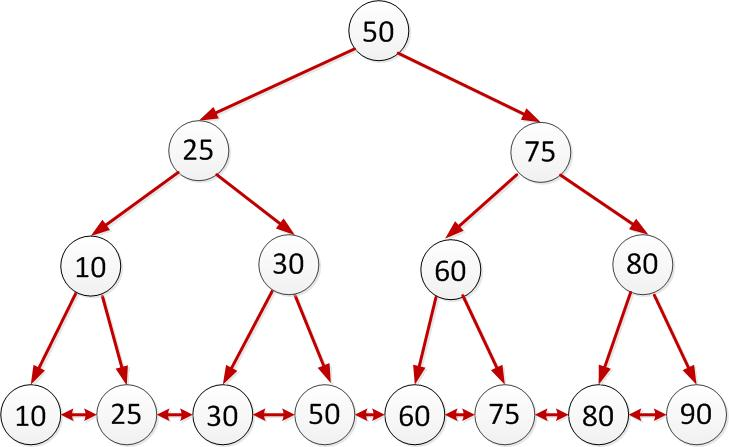
\includegraphics[width=6in, height=2.75in]{Figures/Figure23}}
  \end{center}
  \centering
	\parbox{6in}{\caption{Optimized balanced AVL tree.} \label{fig23}}
\end{figure}

These pointers would be gradually built as the tree grows and there is no separate routine which will update these pointers. These pointers building/ maintaining operation would be built in the tree formation itself. The only thing we should be careful is to update these pointer whenever a node is inserted into or deleted from the tree. Suppose we inserted a new node 55 in between 50 and 60 then the right pointer of 50 and left pointer of 60 should point to 55. At the same time the left pointer of 55 should point to 50 and the right pointer of 55 should point to 60 (Figure.~\ref{fig24}). Similarly while deleting node 55 which was inserted in previous step we need to make sure that right pointer of node 50 points to 60 and the left node of point 60 points to 50.
\begin{figure}[ht]
  \begin{center}
   	\fbox{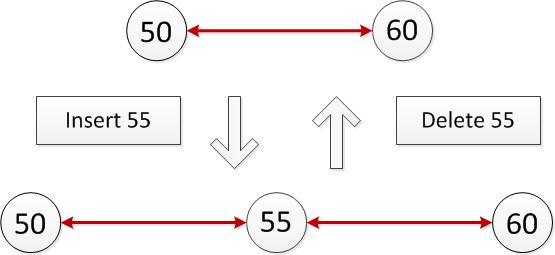
\includegraphics[width=6in, height=1.75in]{Figures/Figure24}}
  \end{center}
  \centering
	\parbox{5in}{\caption{Inserting a leaf in-between two leaves in an optimized AVL tree.} \label{fig24}} 
\end{figure}

\section{Tree rotations}
Remember, we need to perform tree rotations when the tree is not balanced in order to balance it. We perform left or right rotation or a combination of both in a certain order in order to balance the tree. Initially it may seem that maintaining these proposed tree pointers would be a night mare when the tree rotation(s) is performed. All the left and right pointers would seem to be messed when the tree is rotated. Surprisingly, as a matter of fact we do not need to do any special operation when the tree is rotated. If we recall the rules stated for performing tree rotations as given below.
\begin{enumerate}
	\item The order of the leaves prior to rotation and post rotation must remain the same. In other words the order of the leaves in the depth first search should remain the same before and after the rotation.
	\item For any particular node the right child must always be greater than or equal to the parent node and the left child must be less than the parent node. This is the basic property of a binary search tree that needs to be followed by tree rotations.
\end{enumerate}

The first rule is the answer to the question that we just presented. The tree rotation follows the order of the leaves of the tree from left to right or vice-versa. Thus the tree rotation should just work as is without modifying it. If the leaves of the tree maintain the order pre and post rotation then there is no need to update the left and right pointers maintained in the leaves of the tree.

\section{Good Geometric Algorithm}

What makes a geometry algorithm good?  One factor is that it correctly solves a significant problem.  If an algorithm is the very first one or the only one to solve a certain problem, then that alone would make it significant.  Otherwise, something else has to distinguish it.  The primary theoretical  criterion used to compare algorithms is their efficiency, especially their asymptotic efficiency (aka ``computational complexity") as the size n of the problem involved becomes increasingly large,  given by Table \ref{tab3} \cite{SOFTSURFER}.  That is, the algorithm has to be ultimately faster than the competition.  Beyond speed, additional secondary criteria for good algorithms include: the amount of storage space they use, their runtime efficiency for low values of n, their ease of implementation, and also the sheer elegance of the algorithm's solution.  In some cases, the secondary criteria can outweigh the primary one.  For example, in a 1990 tour-de-force, Chazelle described a linear time {\it O}(n) algorithm for triangulating a simple polygon in the plane \cite{Chazelle}.
\begin{table}[hbt]
  \begin{minipage}{6in}
    \caption{Time Complexity of An Algorithm For Input `n'\label{tab3}}
    \begin{tabular}{||p{1.5cm}|p{2cm}|p{2cm}|p{2cm}|p{2cm}|p{2cm}|p{2cm}||}    \hline
      logn & n & nlog n & $n^{2}$ & $n^{3}$ & $n^{4}$ & $2^{n}$ \\ \hline \hline
      0 & 1 & 0 & 1 & 1 & 1 & 2 \\ \hline
	  1 & 2 & 2 & 4 & 8 & 16 & 4 \\ \hline
	  2 & 4 & 8 & 16 & 64 & 256 & 16 \\ \hline
	  3 & 8 & 24 & 64 & 512 & 4096 & 256 \\ \hline
	  4 & 16 & 64 & 256 & 4096 & 65536 & 65536 \\ \hline
	  5 & 32 & 160 & 1024 & 32768 & 1048576 & 4294967296 \\ \hline
	  6 & 64 & 384 & 4096 & 262144 & 16777216 & xxxxxxxxxx \\ \hline
	  7 & 128 & 896 & 16384 & 2097152 & 268435456 &  \\ \hline
	  8 & 256 & 2048 & 65536 & 16777216 & 4294967296 &  \\ \hline
	  9 & 512 & 4608 & 262144 & 134217728 & xxxxxxxxxx &  \\ \hline
	  10 & 1024 & 10240 & 1048576 & 1073741824 &  &  \\ \hline
	  15 & 32768 & 491520 & 1073741824 & xxxxxxxxxx &  &  \\ \hline
	  20 & 1048576 & 20971520 & xxxxxxxxxx &  &  &  \\ \hline
	  25 & 33554432 & 838860800 &  &  &  &  \\ \hline
	\end{tabular}
	\begin{minipage}{1.09\linewidth}
  \begin{tablenotes}[para, flushleft] Source: SOFTSURFER, \textit{Softsurfer}. Geometry Algorithms, \newline http://www.softsurfer.com/overview.htm, accessed Aug. 2012, n.d.
  \end{tablenotes}
  \end{minipage}
  \end{minipage}
\end{table}
However, to this day that algorithm has never been implemented because it is too complicated!  So, other triangulation algorithms that are both reasonably fast and easy to implement become significant.  On the other hand, finding a way to simplify Chazelle's algorithm and actually programming it would be of great significance \cite{SOFTSURFER}.

\section{Space Complexity}

We would need to have extra space of two double words (DWORD), In other words we would need to have 8 bytes $=$ 64 bits for each leaf node in order to save the left and right pointers. Thus in total we would need 64 $*$ n bits more or 8 $*$ n bytes than the original implementation. The important point is that we only store the left and right pointers in the leaf nodes and hence we don`t need the extra space for the internal nodes. Also conceptually the internal nodes should only store the information required to guide the search. The time that we save by following this approach certainly accounts for the extra space.

\section{Time Complexity}

This new approach to save the extra left and right pointers would take constant time to be maintained as they are gradually built as the tree grows. There is no separate dedicated method or loops which will maintain these pointers. They are built into the algorithm and hence would be constant which we can ignore. 
The neighbor search operation for a typical AVL tree takes {\it O}(log n) time \cite{BST}. The neighbor search operation in the optimized mode of the algorithm requires to access the value stored in the left and right pointers only. Thus these are primitive operation and does not include any kind of loops or accessing complex data structures. Hence the neighbor search operation in the optimized mode of the algorithm would require constant time {\it O}(1) time. Thus it is clearly a huge improvement especially for large trees. This would save tremendous amount of time in finding the neighbor when this algorithm is used in some real world application, where the number of input lines are huge.
